\chapter{Schematic Diagram}
The schematic diagram of the system is given below. Here, I have used 5 sensors, 1 GSM-GPRS modem, 1 arduino mega and power supply.
\begin{figure}[hbt!]
 \centering
 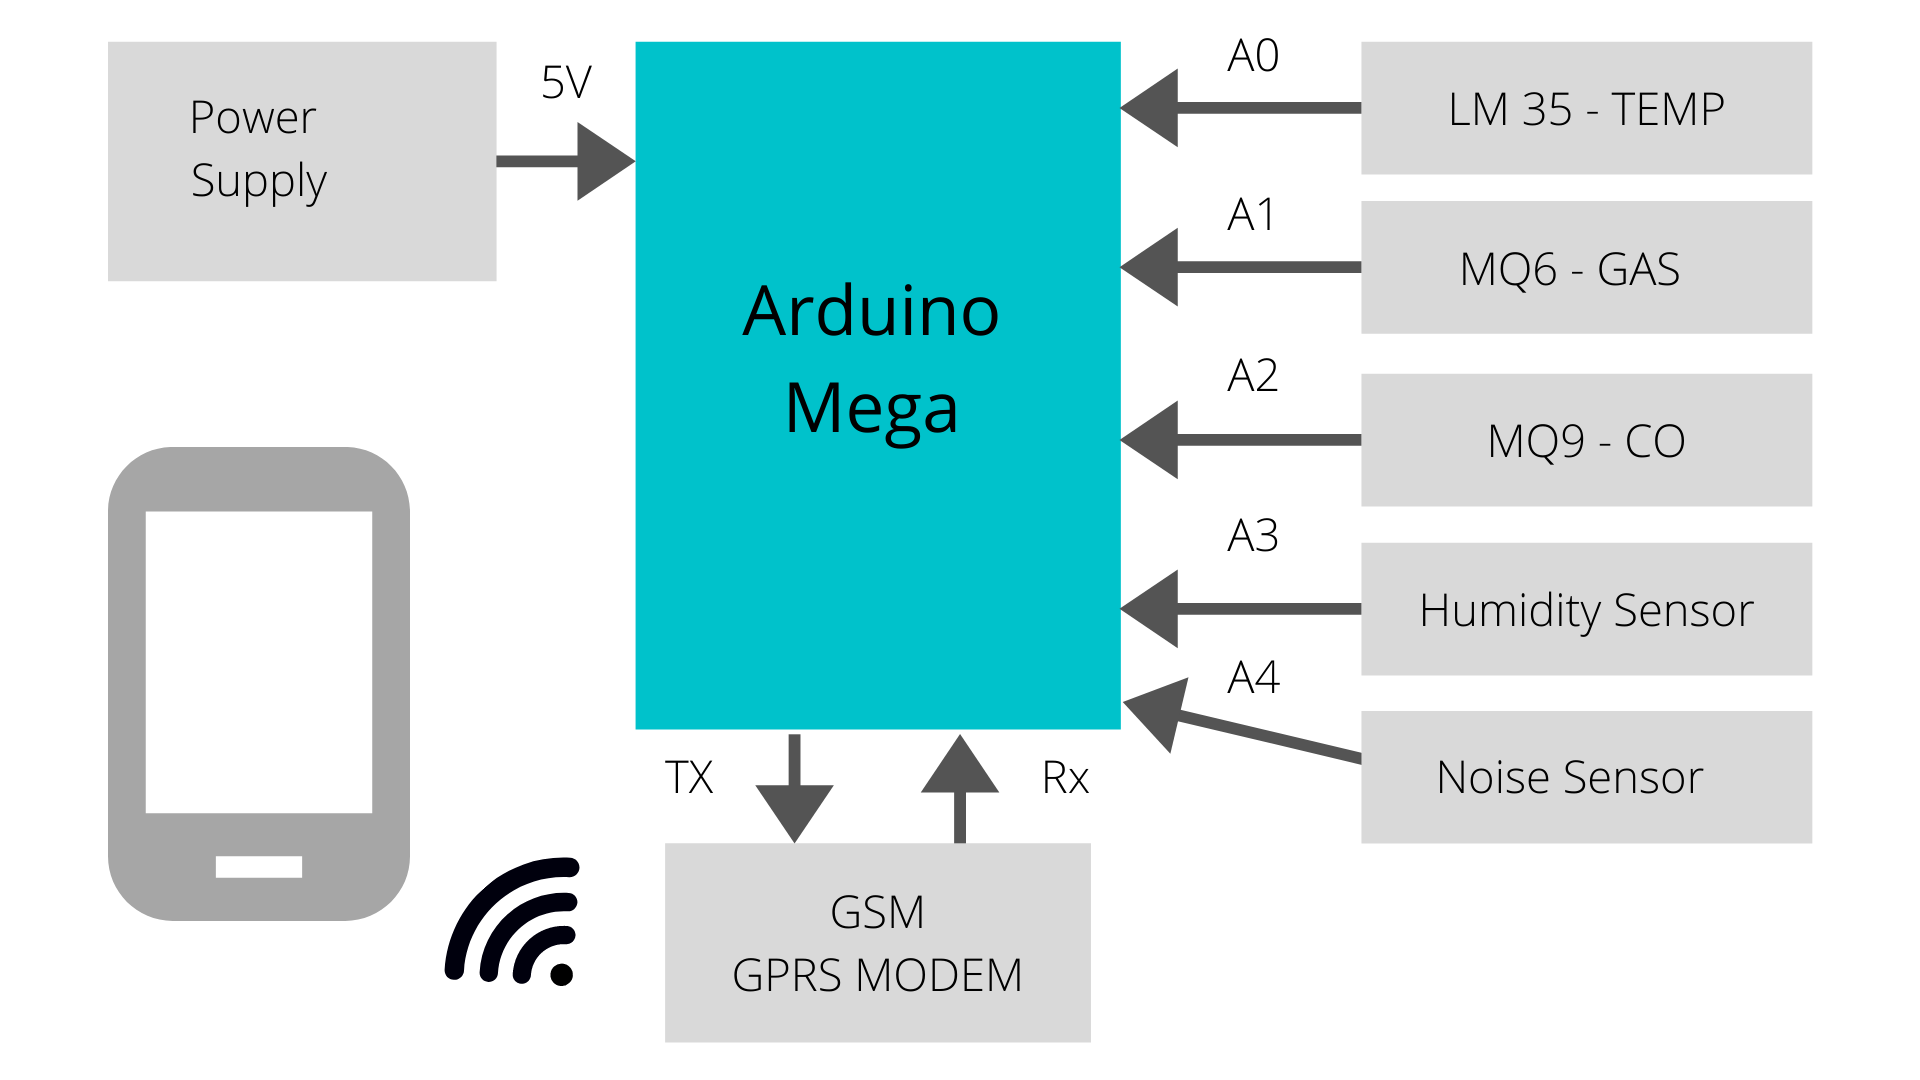
\includegraphics[width=17cm]{title/LM 35 -TEMP.png}
 \caption[]{Schematic Diagram of IoT Based System}
    \label{}
\end{figure}
We have used temperature sensor, gas sensor, $CO$ sensor, humidity sensor and noise sensor.\cite{WinNT} These sensors measures the surrounding conditions and sends the data to the micro-controller. Then the micro-controller sends the data to my device through GSM-GPRS modem. And there is a power supply to the system which is of 5 volt. By this way I can get the information about my surroundings from this system. 